% \iffalse
\let\negmedspace\undefined
\let\negthickspace\undefined
\documentclass[journal,12pt,twocolumn]{IEEEtran}
\usepackage{cite}
\usepackage{amsmath,amssymb,amsfonts,amsthm}
\usepackage{algorithmic}
\usepackage{graphicx}
\usepackage{textcomp}
\usepackage{xcolor}
\usepackage{txfonts}
\usepackage{listings}
\usepackage{enumitem}
\usepackage{mathtools}
\usepackage{gensymb}
\usepackage{comment}
\usepackage[breaklinks=true]{hyperref}
\usepackage{tkz-euclide} 
\usepackage{listings}
\usepackage{gvv}                                        
\def\inputGnumericTable{}                                 
\usepackage[latin1]{inputenc}                                
\usepackage{color}                                            
\usepackage{array}                                            
\usepackage{longtable}                                       
\usepackage{calc}                                             
\usepackage{multirow}                                         
\usepackage{hhline}                                           
\usepackage{ifthen}                                           
\usepackage{lscape}

\newtheorem{theorem}{Theorem}[section]
\newtheorem{problem}{Problem}
\newtheorem{proposition}{Proposition}[section]
\newtheorem{lemma}{Lemma}[section]
\newtheorem{corollary}[theorem]{Corollary}
\newtheorem{example}{Example}[section]
\newtheorem{definition}[problem]{Definition}
\newcommand{\BEQA}{\begin{eqnarray}}
\newcommand{\EEQA}{\end{eqnarray}}
\newcommand{\define}{\stackrel{\triangle}{=}}
\theoremstyle{remark}
\newtheorem{rem}{Remark}
\begin{document}
\parindent 0px
\bibliographystyle{IEEEtran}
\title{GATE: CH - 45.2023}
\author{EE22BTECH11219 - Rada Sai Sujan$^{}$% <-this % stops a space
}
\maketitle
\newpage
\bigskip
\section*{Question}
Level \brak{h} in a steam boiler is controlled by manipulating the flow rate \brak{F} of the break-up(fresh) water using a proportional \brak{P} controller. The transfer function between the output and the manipulated input is   \\
$$ \frac{h\brak{s}}{F\brak{s}}=\frac{0.25\brak{1-s}}{s\brak{2s+1}} $$   \\
The measurement and the valve transfer functions are both equal to 1. A process engineer wants to tune the controller so that the closed loop response gives the decaying oscillations under the servo mode. Which one of the following is the CORRECT value of the controller gain to be used by the engineer? \\
\begin{enumerate}[label=(\alph*)]
    \item $0.25$
    \item $2$
    \item $4$
    \item $6$
\end{enumerate}
\solution
\begin{table}[ht]
    \centering
    \begin{tabular}{|p{2cm}|p{2cm}|p{3.8cm}|}
    \hline
    PARAMETER & VALUE  & DESCRIPTION \\ \hline
    $$G_c$$ & $$K_c$$ & Proportional controller's transfer function \\ \hline
    $$G_f$$ & $$1$$ & Valve transfer function \\ \hline
    $$G_p$$ & $$\frac{0.25\brak{1-s}}{s\brak{2s+1}}$$ & Process transfer function   \\ \hline
    $$G_M$$ & $$1$$ & Measurement transfer function \\ \hline 
    \end{tabular}

    \caption{PARAMETER TABLE 1}
    \label{tab:ch.45.1}
\end{table} \\
\begin{figure}[ht]
    \centering
    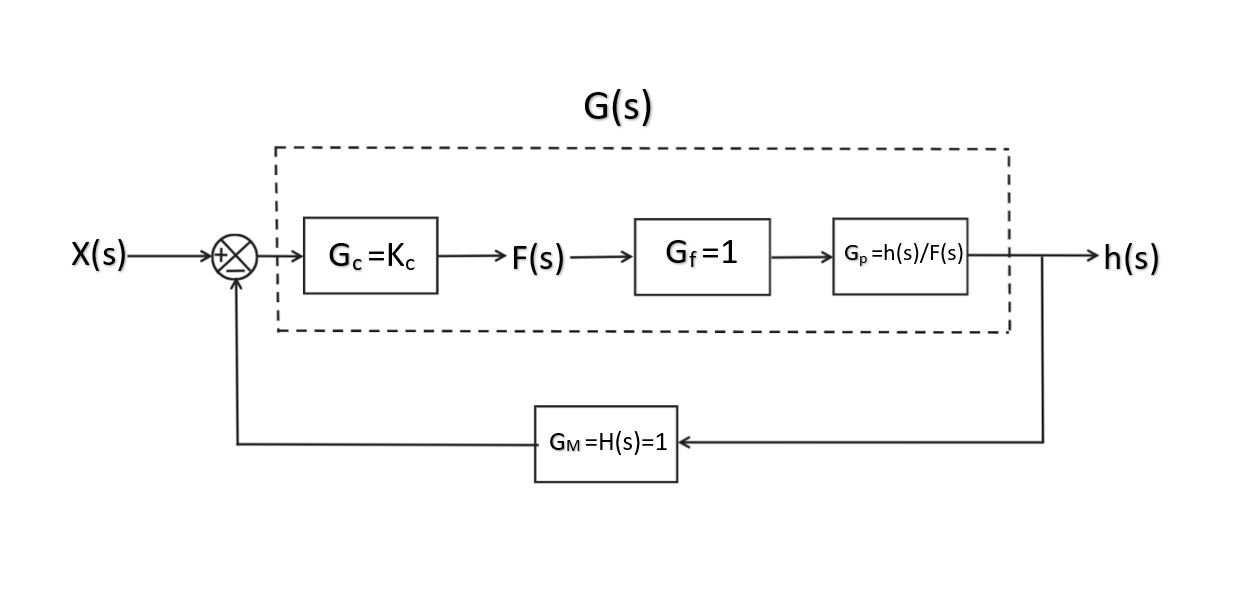
\includegraphics[width=\columnwidth]{figs/k.png}
    \caption{Closed loop Block diagram}
    \label{fig:ch.45.1}
\end{figure}    \\
Closed loop signal transfer function of the above block diagram can be given by,
\begin{align}
     T\brak{s} &= \frac{G\brak{s}}{1+G\brak{s}H\brak{s}}    
\end{align}
From \figref{fig:ch.45.1} and \tabref{tab:ch.45.1}
for a unit impulse, $X\brak{s}=1$ \\
\begin{align}
    h\brak{s} &= T\brak{s}\times X\brak{s}   \\
    h\brak{s} &= \frac{\brak{1-s}K_c}{8s^2 + \brak{4-K_c}s + K_c}  \\
    \implies h\brak{s} &= \frac{\brak{1-s}K_c}{8\brak{s-s_1}\brak{s-s_2}}  \label{eq:ch.45.4}
\end{align}
Where,
\begin{align}
    s_1 &= \frac{\brak{K_c-4}}{16} + \sqrt{\brak{\frac{K_c-4}{16}}^2 - \frac{K_c}{8}}  \\
    s_2 &= \frac{\brak{K_c-4}}{16} - \sqrt{\brak{\frac{K_c-4}{16}}^2 - \frac{K_c}{8}} 
\end{align}
From \eqref{eq:ch.45.4} we get,
\begin{align}
    h\brak{s} &= \frac{K_c}{8\brak{s_1-s_2}}\brak{\frac{1-s_1}{s-s_1}-\frac{1-s_2}{s-s_2}}
\end{align}
Now taking the inverse laplace transform we have,
\begin{align}
    h\brak{t} &= \frac{K_c}{8\brak{s_1-s_2}} \left [\brak{1-s_1}e^{s_1t}-\brak{1-s_2}e^{s_2t} \right ]u\brak{t}  \\
    \implies h\brak{t} &= e^{\frac{K_c-4}{16}}\brak{A_1e^{\sqrt{\brak{\frac{K_c-4}{16}}^2 - \frac{K_c}{8}}} - A_2e^{-\sqrt{\brak{\frac{K_c-4}{16}}^2 - \frac{K_c}{8}}}}u\brak{t}    
\end{align}
Where,
\begin{align}
    A_1 &= \frac{K_c}{8} \brak{\frac{1-s_1}{s_1-s_2}}    \\
    A_2 &= \frac{K_c}{8} \brak{\frac{1-s_2}{s_1-s_2}}    
\end{align}
Now applying the condition for underdamped oscillations,
\begin{align}
    \brak{\frac{K_c-4}{16}}^2 - \frac{K_c}{8} < 0    \\
    \implies K_c \in \brak{20-\sqrt{384} , 20+\sqrt{384}}   \label{eq:ch.45.13}
\end{align}
For the system to be stable,
\begin{align}
    \frac{K_c-4}{8}&<0   \\
    \implies K_c&<4 	\label{eq:ch.45.15}
\end{align}
From \eqref{eq:ch.45.13} and \eqref{eq:ch.45.15}
\begin{align}
    &K_c \in \brak{0.4,4}    \label{eq:ch.45.16}
\end{align}
\eqref{eq:ch.45.16} represents the $ROC$,$(R_e\{s\}<0)$
\begin{align}
    \implies &K_c=2
\end{align}
\begin{figure}[htbp]
    \centering
    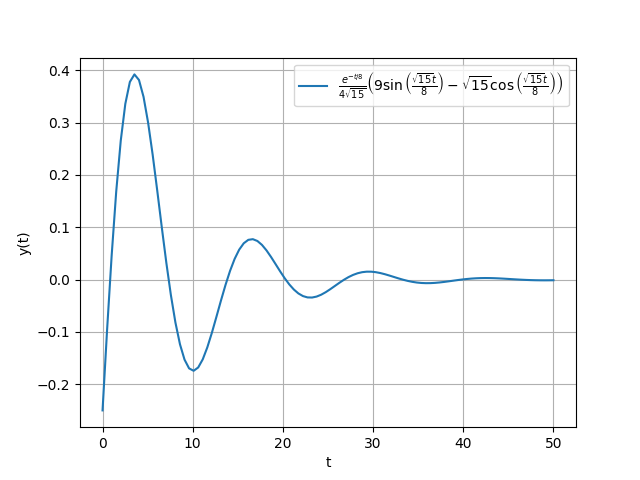
\includegraphics[width=\columnwidth]{figs/b.png}
    \caption{y\brak{t} $vs$ t graph}
    \label{fig:ch.45.2}
\end{figure}     
\end{document}
